\documentclass[11pt,a4paper]{article}
\usepackage[utf8]{inputenc}
\usepackage[spanish]{babel}	%Idioma
\usepackage{amsmath}
\usepackage{amsfonts}
\usepackage{amssymb}
\usepackage{graphicx} 	%Añadir imágenes
\usepackage{geometry}	%Ajustar márgenes
\usepackage[export]{adjustbox}[2011/08/13]
\usepackage{float}
\restylefloat{table}
\usepackage[hidelinks]{hyperref}
\usepackage{titling}
\graphicspath{{/home/nazaret/Escritorio/LaTEX}}
%\usepackage{minted}
\usepackage{multirow}
\usepackage{caption}
\usepackage{multicol}
\usepackage[shortlabels]{enumitem}
\usepackage{array}
\selectlanguage{spanish}

%Opciones de encabezado y pie de página:
\usepackage{fancyhdr}
\pagestyle{fancy}
\lhead{Nazaret Román Guerrero}
\rhead{Procesamiento Digital de Señales}
\lfoot{Grado en Ingeniería Informática}
\cfoot{}
\rfoot{\thepage}
\renewcommand{\headrulewidth}{0.4pt}
\renewcommand{\footrulewidth}{0.4pt}

%Opciones de fuente:
\usepackage[utf8]{inputenc}
\usepackage[default]{sourcesanspro}
\usepackage{sourcecodepro}
\usepackage[T1]{fontenc}

\setlength{\parindent}{15pt}
\setlength{\headheight}{15pt}
\setlength{\voffset}{10mm}

% Custom colors
\usepackage{color}
\definecolor{deepblue}{rgb}{0,0,0.5}
\definecolor{deepred}{rgb}{0.6,0,0}
\definecolor{deepgreen}{rgb}{0,0.5,0}

\usepackage{listings}
\usepackage{color}
\usepackage{graphicx}

\definecolor{dkgreen}{rgb}{0,0.6,0}
\definecolor{gray}{rgb}{0.5,0.5,0.5}
\definecolor{mauve}{rgb}{0.58,0,0.82}

\lstset{frame=tb,
  language=Matlab,
  aboveskip=3mm,
  belowskip=3mm,
  showstringspaces=false,
  columns=flexible,
  basicstyle={\small\ttfamily},
  numbers=left,
  numberstyle=\tiny\color{gray},
  keywordstyle=\color{blue},
  commentstyle=\color{dkgreen},
  stringstyle=\color{mauve},
  breaklines=true,
  breakatwhitespace=true,
  tabsize=4
}

\begin{document}
\begin{titlepage}

\begin{minipage}{\textwidth}

\centering

\includegraphics[width=0.55\textwidth]{logo.png}\\

\textsc{\Large Procesamiento Digital de Señales\\[0.2cm]}
\textsc{GRADO EN INGENIERÍA INFORMÁTICA}\\[1cm]

{\Huge\bfseries Relación de ejercicios\\}
\noindent\rule[-1ex]{\textwidth}{3pt}\\[3.5ex]
{\large\bfseries Ejercicios de teoría. Tema 1}
\end{minipage}

\vspace{1.5cm}
\begin{minipage}{\textwidth}
\centering

\textbf{Autora}\\ {Nazaret Román Guerrero}\\[2.5ex]

\includegraphics[width=0.3\textwidth]{etsiit.jpeg}\\[0.1cm]
\vspace{1cm}
\textsc{Escuela Técnica Superior de Ingenierías Informática y de Telecomunicación}\\
\vspace{1cm}
\textsc{Curso 2018-2019}
\end{minipage}
\end{titlepage}

\pagenumbering{gobble}
\pagenumbering{arabic}
\tableofcontents
\thispagestyle{empty}

\newpage

\section{Ejercicio 1}

La señal en tiempo discreto

\[x(n)=6.35cos(\pi n/10) \]

es cuantizada con una resolución: (a) $\Delta = 0.1$ o (b) $\Delta = 0.02$. ¿Cuántos bits necesita el convertidor A/D en cada caso?\\ \\



Para calcular los bits necesarios vamos a utilizar la ecuación de la cuantización.

\begin{enumerate}[a)]
	\item $\Delta = 0.1$
	
	\begin{gather*}
	Delta = \frac{2X_{max}}{2^B} \\
	2^B = \frac{2X_{max}}{\Delta} = \frac{2*6.35}{0.1} = 127
	\end{gather*}

Ahora solo debemos calcular el logaritmo para sacar los bits que necesita el cuantizador.

	\[B = log_2(127) = 6.98\sim 7\]
	
Puesto que el cuantizador no puede tener 6.98 bits, lo redondeamos hacia arriba. Por lo tanto, el cuantizador necesitará 7 bits para poder cuantizar 127 valores, y sobrará un valor que no necesita para cuantizar ningún valor.
	
	\item $\Delta = 0.02$
	
	Ahora vamos a calcularlo para el segundo caso haciendo lo mismo que hemos hecho en el otro caso.
	
	\begin{gather*}
	Delta = \frac{2X_{max}}{2^B} \\
	2^B = \frac{2X_{max}}{\Delta} = \frac{2*6.35}{0.02} = 635
	\end{gather*}

	\[B = log_2(635) = 9.31\sim 10\]
	
En este caso necesita 10 bits aunque de los 1024 valores disponibles solo utilizará 635.
\end{enumerate}

\newpage

\section{Ejercicio 19}

Una señal analógica de electrocardiograma (ECG) contiene frecuencias hasta 100 Hz.

\begin{enumerate}[a)]
	\item Determine la frecuencia de Nyquist para esta señal.
	\item Suponga que muestreamos esta señal a una frecuencia de 250 muestras/s. Determine el valor de la frecuencia más alta de la señal ECG que se puede representar correctamente a esta frecuencia de muestreo.\\
\end{enumerate}



Para calcular este ejercicio vamos a hacer uso del \textbf{Teorema de muestreo}.

\begin{enumerate}[a)]
	\item Frecuencia de Nyquist.

	Como sabemos, la frecuencia de muestreo debe ser al menos igual al doble de la frecuencia máxima de la señal analógica, que se corresponde con la frecuencia de Nyquist. Es decir:
	
	\[f_s \geq 2f_{max}\]
	
	donde $2f_{max} = f_{Nyquist}$. Por tanto tenemos que
	
	\[2\cdot 100 = f_{Nyquist}\]
	
	Es decir, la frecuencia de Nyquist es 200 muestras/s.
		
	\item Frecuencia máxima con $f_s = 250$ muestras/s.
	
	En este caso sabemos que la frecuencia de muestreo es de 250, por lo que solo necesitamos calcular la frecuencia máxima que podría tener el ECG que fuera correctamente registrada.
	
	\begin{gather*}
	f_s \geq 2f_{max} \Rightarrow 250 \geq 2f_{max}\\
	f_{max} = \frac{250}{2} = 125
	\end{gather*}
	
	Por tanto sabemos que el ECG podría tener una frecuencia máxima de 125 Hz.
\end{enumerate}

\newpage

\section{Ejercicio 20}

Se muestrea una señal analógica $x_a(t) = sin(480\pi t) + 3sin(720\pi t)$ a una frecuencia de 600 muestras por segundo.
\begin{enumerate}[a)]
	\item Determine la frecuencia de Nyquist para la señal $x_a(t)$.
	\item Determine las frecuencias, en radianes, de la señal discreta resultante $x(n)$.
	\item Si se hace pasar $x(n)$ a través de un convertidor D/A ideal, ¿cuál sería la señal reconstruida $y_a(t)$?\\
\end{enumerate}



\begin{enumerate}[a)]
	\item Para resolver este apartado vamos a utilizar el Teorema de muestreo. Primero necesitamos saber las frecuencias a las que puede llegar la señal. Sabemos que
	
	\[\omega = 2\pi f\]
	
	Por lo que vamos a calcular $f_1$ y $f_2$:

	\begin{gather*}
	\omega = 2\pi f_1;\\
	f_1 = \frac{\omega}{2\pi} = \frac{480\pi}{2\pi} = 240
	\end{gather*}
	
	La primera frecuencia es 240 Hz. Vamos a calcular la segunda y veremos cuál es la máxima.
	
	\begin{gather*}
	\omega = 2\pi f_2;\\
	f_2 = \frac{\omega}{2\pi} = \frac{720\pi}{2\pi} = 360
	\end{gather*}
	
	La segunda frecuencia es 360 Hz que se corresponde con la máxima. Así que ahora vamos a utilizar el Teorema de muestreo con esta frecuencia que acabamos de calcular. Sabiendo que la frecuencia de Nyquist es el doble de la frecuencia máxima:
	
	\[f_{Nyquist} = 2f_{max} = 2\cdot 360 = 720\]
	
	Es decir, la frecuencia de Nyquist es 720 Hz, lo que significa que la señal se está muestreando sin cumplir el Teorema de muestreo, ya que la frecuencia de muestreo es $F_s=600$ Hz, menor que el doble de la frecuencia máxima de la señal analógica.
	
	\item Puesto que no estamos muestreando correctamente, todas aquellas frecuencias que sean mayores que 600 Hz no las vamos a poder detectar, por lo tanto, la ecuación de la señal muestreada es:
	
	\[x(n) = sin\left( \frac{480\pi n}{600}\right) \]
	
	Por tanto, la frecuencia máxima de la señal muestreada es $f_{max} = \frac{480\pi}{600} = \frac{4\pi}{5}$.
	
	\item Finalmente vamos a reconstuir la señal a partir de la señal muestreada. Debido a que no se ha muestreado correctamente, se pierden frecuencias, en concreto todas aquella que estén por encima de 600 Hz. Si reducimos el rango entre $-F_s/2$ y $F_s/2$, se toman las frecuencias entre -300 y 300, lo que significa que la frecuencia máxima no se va a registrar ya que tiene una frecuencia de 360 Hz.\\
	
	La señal real es algo como lo siguiente:
	
	\begin{figure}[H]
		\centering
		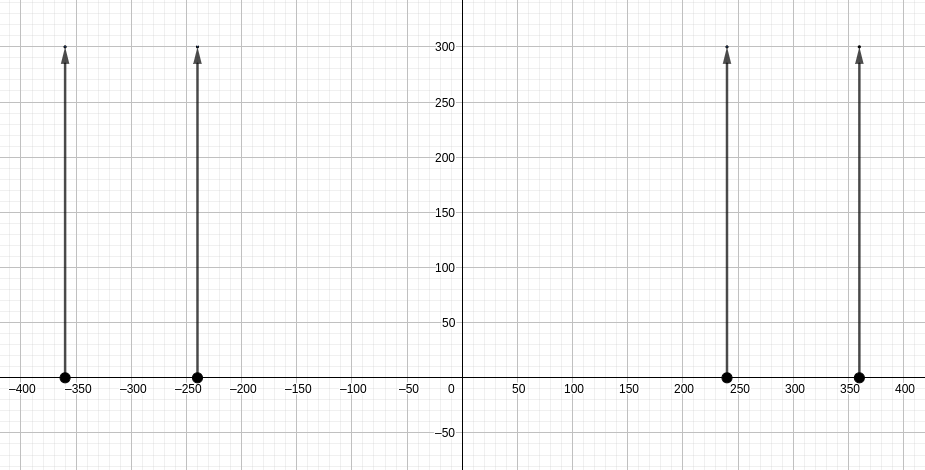
\includegraphics[scale=0.3]{original.png}
	\end{figure}
	
	Al muestrear a 600 Hz 
	
	\begin{figure}[H]
		\centering
		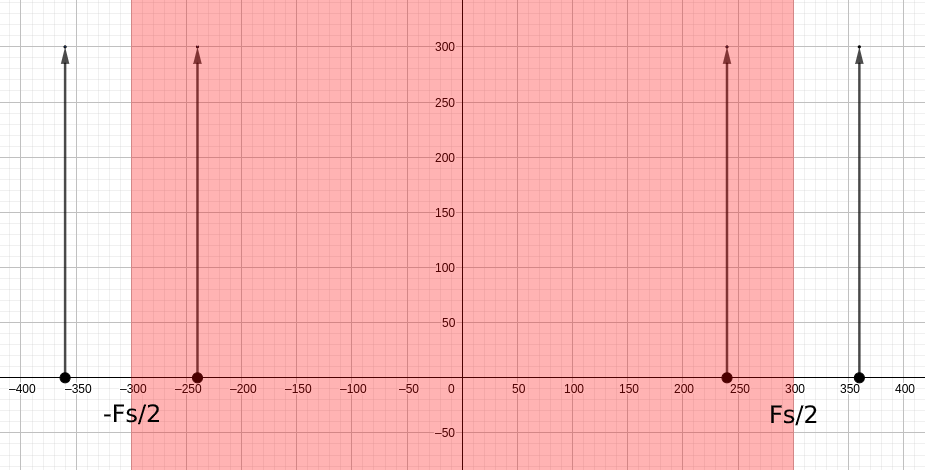
\includegraphics[scale=0.3]{muestreada.png}
	\end{figure}
	
	Donde la parte roja indica la parte que se mantiene, mientras que el resto queda fuera del alcance de la frecuencia de muestreo. Esto siginifica que estamos perdiendo componentes de la señal. Por tanto la señal reconstruida queda como:
	
	\[y_a(t) = sin(480\pi t)\]
	
	Es decir, no cumpliendo el Teorema de muestreo perdemos la señal original y no seremos capaces de recuperarla.
	
\end{enumerate}

\end{document}